
%(BEGIN_QUESTION)
% Copyright 2008, Tony R. Kuphaldt, released under the Creative Commons Attribution License (v 1.0)
% This means you may do almost anything with this work of mine, so long as you give me proper credit

A digital computer network uses a two-conductor cable to send both power (DC) and data (AC pulses) from one computer to another, inductors and capacitors being used to filter the voltages to and from their proper sources and destinations:

$$\includegraphics[width=15.5cm]{i03171x01.eps}$$

The system works fine for a while, but then one day the receiving computer stops receiving data.  It still has DC power getting to it, but just no digital data.  Identify the following:

\vskip 10pt

\begin{itemize}
\item{} \underbar{One} failed component in the circuit that could possibly account for the problem, and the type of fault (open or short) you suspect that component would have.
\vskip 40pt
\item{} Show where you would connect a voltmeter in the circuit to verify a fault in that one suspect component, and the voltage reading (AC, DC, or both) you would expect to get if indeed that one component had failed.
\end{itemize}

\vfil 

\underbar{file i03171}
\eject
%(END_QUESTION)





%(BEGIN_ANSWER)

This is a graded question -- no answers or hints given!

%(END_ANSWER)





%(BEGIN_NOTES)

Since the receiving computer is still receiving DC power from the sending computer just like it's supposed to, we know the cable is not faulted either open or shorted.  This leaves only the AC signaling components under suspicion.

\vskip 10pt

\noindent
{\bf Possible component faults, and their respective validating tests}

\begin{itemize}
\item{} Source $V_1$ failed (no signal); measure 0 AC voltage directly across its terminals.
\item{} Problem with receiving computer circuitry (digital data load ``resistor'' failed open); measure full AC voltage directly across its terminals.
\item{} Capacitor $C_1$ failed open; measure full AC voltage directly across its terminals.
\item{} Capacitor $C_2$ failed open; measure full AC voltage directly across its terminals.
\item{} Capacitor $C_3$ failed open; measure full AC voltage directly across its terminals.
\item{} Capacitor $C_4$ failed open; measure full AC voltage directly across its terminals.
\end{itemize}

%INDEX% Troubleshooting review: electric circuits

%(END_NOTES)


